%!TEX root = ../paper.tex

\section{Smart Restaurant Experience}
\label{sec:smart_restaurant_experience}
% Normal restaurant experience
% Smart restaurant experience
% For waiters
% For customers
% Figures: Smart restaurant from wiki
% -> Screenshots?

Since we aim to improve restaurants' service, we need to compare our approach
with what usually happens. ??
Usually, the customer arrives at the restaurant, get a sit and calls a waiter
to place his order. However, the waiter can be busy processing orders
from other customers, which can delay this new order.
Figure~\ref{fig:smart_restaurant} shows the interactions between the
customer and the waiter in a normal restaurant (on the left) and in
a smart restaurtant (on the right). It is possible to see that our
solution removes some interactions. For instance, the customer does not
need to wait until he is able to place his order.
The main goal is not to replace the workers but instead help them to do a
better job.
There are three groups of users of the solution being proposed here:

\begin{description}
  \item[Waiters] who will use a web application to see the customers'
  orders;
  \item[Owners] who will use a mobile app to configure the
  restaurants' menu and the mapping between the tables and the beacons;
  \item[Customers] who will use a mobile app (not the same app as the
  Owners use) that will notify him when he arrives at the restaurant and
  will present the menu.
\end{description}

Next, for each kind of user, we will present the main features and their
advantages.

\begin{figure}[!ht]
  \centering
    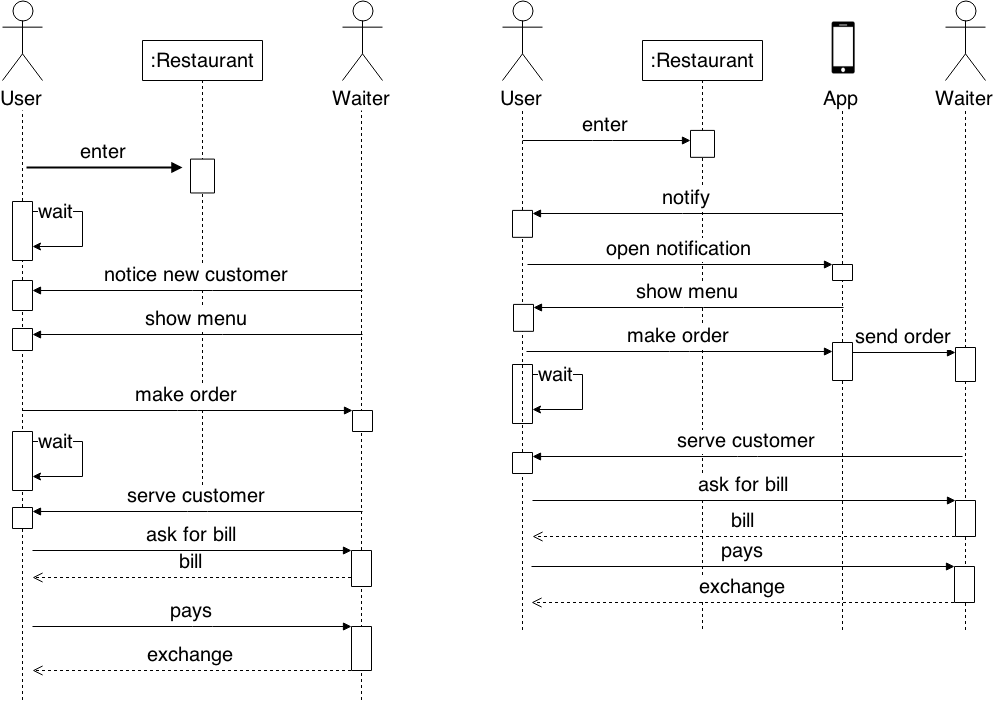
\includegraphics[width=1\textwidth]{figures/smart-restaurant}
    \caption{Sequence diagram showing the interactions between
    the customer and the waiter in a normal restaurant (on the left)
    and in a Smart Restaurant(on the right)}
    \label{fig:smart_restaurant}
\end{figure}

\subsection{Customers}
\label{sub:customers}
As it is shown in figure~\ref{fig:smart_restaurant} some interactions between
the customer and the waiter can be replaced by a mobile app.
For this group of users, the main feature is to allow them to place
the orders using their smartphones. The mobile app detects in which table
the customer is in and sends that information to the web application that the
Owners use. When the customer places his order, he does not need to type
the number of the table. This way, the customer will get his orders
processed faster.

\subsection{Waiters}
\label{sub:waiters}
% Features
This group of users is responsible for processing the customers' orders.
As already mentioned, the smart restaurant solution does not aim to replace
the waiters. It tries to make their job easier. In order to do that,
there is a web application where waiters can check who is requesting them.
Since the mobile app for customers allows them to request a waiter or to place
an order, the web application for waiters allows them to see the customers'
requests. As soon as the customer requests a waiter or place an order,
the web application shows that information and waiters can see from which
table the request is coming from.

\subsection{Owners}
\label{sub:owners}
Before customers and waiters can use this solution, the restaurants' owners
need to do some configurations in order to set everything up.
There is a mobile app for owners that allows them to turn their normal
restaurants in smart ones.
Using this mobile app, owners can configure the menu and the tables.
As already mentioned, this solution uses BLE beacons. To configure
the restaurant's tables, the owners need to perform the following steps:
\begin{itemize}
  \item Deploy one beacon in each table;
  \item Open the mobile app for owners;
  \item Login in the app;
  \item Select the option to configure the tables;
  \item Move the mobile device close to the beacon;
  \item Once the beacon has been detected, select it and type the number
  of the corresponding table
\end{itemize}
Once these steps are done, now they just have to configure the name of the
restaurant and its menu. This menu will be shown to the customers after they
have been notified that they entered in a smart restaurant.
